\documentclass[preprint2]{aastex}

\shorttitle{Q6}
\shortauthors{Chojnowski}

\begin{document}

\title{Q6}

%% Use \author, \affil, and the \and command to format
%% author and affiliation information.
%% Note that \email has replaced the old \authoremail command
%% from AASTeX v4.0. You can use \email to mark an email address
%% anywhere in the paper, not just in the front matter.
%% As in the title, use \\ to force line breaks.

\author{S. Drew Chojnowski}
\affil{Astronomy Department, New Mexico State University}

\vspace{0.5cm}

\section{What I Did}

In the previous question, I failed to complete parts (d) and (e). My function produces the following result for the integral split into 10 pieces...

In [2]: print a.func3(10)

0.0

2578.36817871

4426.45979984

5697.26375145

6525.76688188

7028.9532352

7305.80279474

7437.28921763

7486.37513769

7497.99973247 (final sum)

...which is not getting anywhere close to the analytical answer. I don't know why.

My reaction to non-success in this part is best expressed in Figure~\ref{kittenfig}, which shows a sad little kitten whose mommy is nowhere in sight.


\begin{figure}[h!]
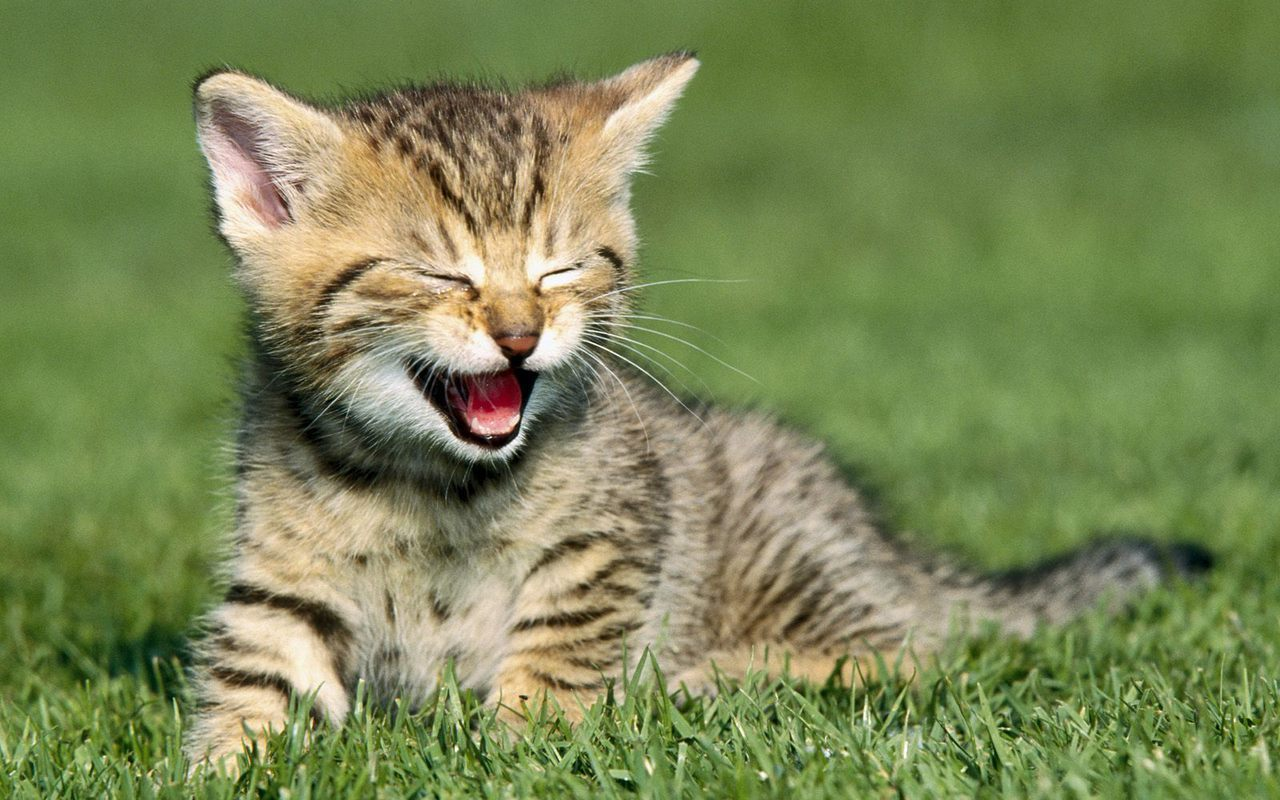
\includegraphics[angle=0,scale=.18]{kitten.jpg}
\caption{Graphical representation of a sad little kitten. \label{kittenfig}}
\end{figure}

\end{document}
